\documentclass[11pt]{article}

\usepackage[margin=1in]{geometry}
\usepackage{booktabs}
\usepackage{graphicx}
\usepackage{amsmath}
\usepackage[hidelinks]{hyperref}
\usepackage{parskip}

\graphicspath{{figures/}}

\title{CUDA Kernel Lab: Driving a GEMM from Naive to Compute Bound on an RTX 5070}
\author{Olajide Badejo}
\date{2026}

\begin{document}
\maketitle

\begin{abstract}
This report documents a CUDA kernel library whose general matrix multiply path is
driven, through explicit optimization steps and Nsight Compute diagnostic rounds,
from a naive baseline to a compute bound tensor core kernel. Every performance
figure is my kernel measured against the vendor library (cuBLAS, or cuSPARSE for
sparse matrix vector) on one GPU, an NVIDIA RTX 5070, in the same process. There
are no cross device comparisons. The top FP16 kernel passes the compute bound gate
and reaches about 90 percent of cuBLAS at 4096 and 8192 cubed. Alongside the GEMM
ladder the library carries GEMV, TRSM, CSR SpMV, and a cuSOLVER wrapper, all
verified against the vendor library, with a measured roofline that places each
kernel against the machine's limits.
\end{abstract}

\section{Introduction}

The aim is narrow on purpose: take one operation, GEMM, and push a hand written
kernel from a fair first pass to the point where Nsight Compute reports it as
compute bound and it lands within about ten percent of cuBLAS on this specific
card. The discipline that makes the result trustworthy is the comparison policy.
Percent of cuBLAS on the same device is the only headline used, because it cancels
the hardware out of the claim. No number in this report comes from anywhere but a
run of this code on this machine, and each is traceable to a results file and a
commit hash.

The machine is an RTX 5070 (Blackwell GB205, compute capability 12.0, sm\_120, 48
SMs, 12 GB GDDR7), running CUDA Toolkit 13.3 inside WSL2. The ceilings used
throughout are measured, not read from the datasheet: about 579 GB/s streaming
bandwidth, 23 TFLOP/s FP32, and 65 TFLOP/s tensor core (best cuBLAS FP16).

\section{Background}

\paragraph{Roofline.} The roofline model bounds attainable performance by
$\min(\text{peak compute}, \text{peak bandwidth} \times \text{arithmetic
intensity})$~\cite{williams2009}. The ridge, peak compute over peak bandwidth,
separates the memory bound region (left) from the compute bound region (right).
GEMM at large $N$ has an arithmetic intensity that grows with $N$, so it lives far
to the right of the ridge; a slow GEMM is therefore an implementation gap, not an
algorithmic ceiling.

\paragraph{Blocking theory.} The decisive step from a shared memory tiled kernel
to a fast one is register blocking: each thread computes many outputs, which lifts
the arithmetic intensity per thread and the work done per shared memory
instruction. This follows Volkov and Demmel~\cite{volkov2008}, and the diagnostic
rounds below confirm it on Blackwell.

\paragraph{Tensor pipeline.} The fifth generation tensor cores raise the compute
ceiling far above the FP32 units. Reaching that ceiling means feeding the cores
fast enough, which is a shared memory problem: the fragment loads, not the matrix
multiply instructions, are what saturate first.

\section{Methodology}

\paragraph{Timing.} Every measurement uses CUDA events with five warmup launches
then twenty timed reps, reported as the median so a single slow rep does not move
the headline. NVML samples power, clocks, temperature, and throttle reasons on a
background thread during every sweep; a throttled run is rerun after cooldown
rather than reported.

\paragraph{Diagnostic rounds.} After each ladder rung, one Nsight Compute round:
capture the Speed of Light, occupancy, memory workload, and warp stall reasons;
name the top limiter; state a hypothesis; apply exactly one change; re-measure.
Each round is one dated entry backed by an ncu report. This loop, not any single
kernel, is the method.

\section{GEMM design and optimization}

The ladder exists so the benchmark table attributes each gain to a cause. Table
\ref{tab:ladder} and Figure \ref{fig:ladder} give the measured result at 4096
cubed; the narrative below is the diagnostic log in brief.

\begin{table}[htbp]
\centering
\begin{tabular}{llrr}
\toprule
rung & precision & GFLOP/s & percent of cuBLAS \\
\midrule
naive & fp32 & 1908 & 8.7 \\
shared tiled & fp32 & 1584 & 7.4 \\
register blocked & fp32 & 10390 & 47.1 \\
cp.async double buffered & fp32 & 16210 & 73.5 \\
WMMA & fp16 & 36333 & 59.3 \\
mma.sync PTX & fp16 & 36343 & 59.5 \\
mma.sync + ldmatrix & fp16 & 36550 & 59.8 \\
mma.sync + ldmatrix + swizzle & fp16 & 54985 & 89.9 \\
WMMA (BF16) & bf16 & 33563 & 53.4 \\
\bottomrule
\end{tabular}

\caption{GEMM ladder at 4096 cubed, each rung versus cuBLAS of the same precision,
measured on the RTX 5070.}
\label{tab:ladder}
\end{table}

\begin{figure}[htbp]
\centering
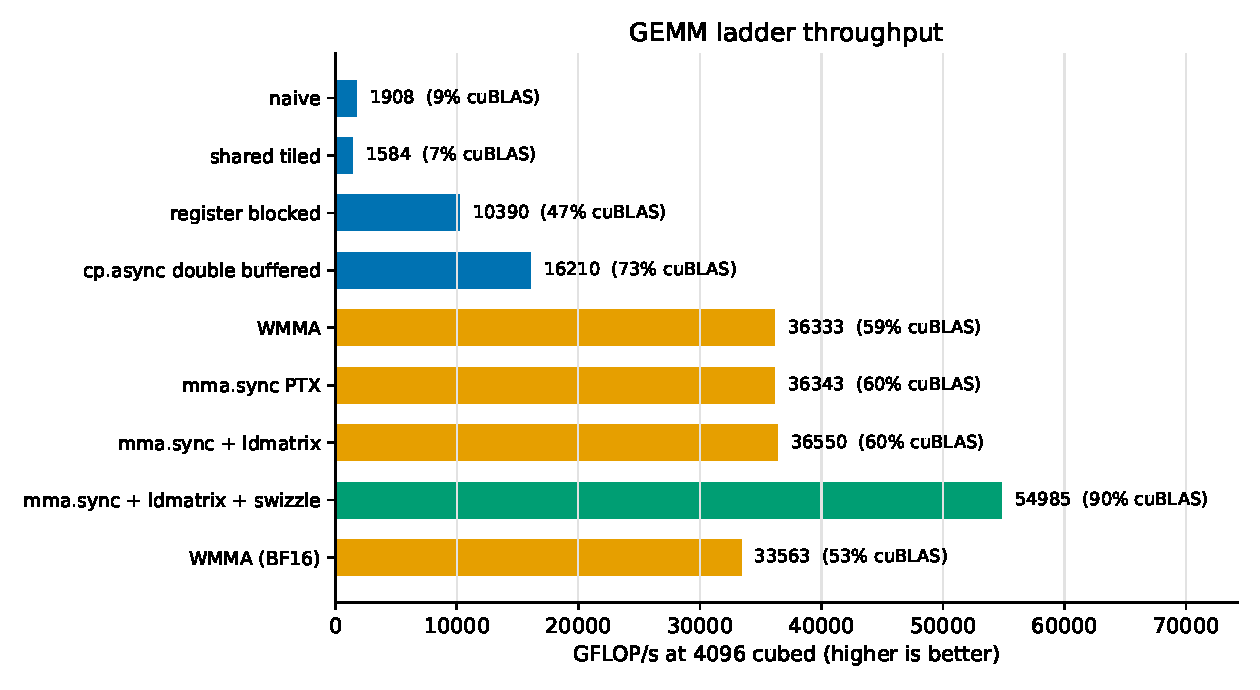
\includegraphics[width=0.9\textwidth]{ladder.pdf}
\caption{GEMM ladder throughput at 4096 cubed. FP32 rungs in blue, tensor rungs in
amber, the top kernel in green.}
\label{fig:ladder}
\end{figure}

\paragraph{Naive to tiled (Round 1).} The naive kernel reaches about 1.9 TFLOP/s.
The shared memory tiled kernel is, surprisingly, slightly slower. The round names
the cause: the tiled 32 by 32 block is 1024 threads, so only one block fits per SM
(about 66 percent occupancy against 100 percent for naive), and its top stall is
the MIO (shared memory) pipe. Meanwhile the naive kernel is not bandwidth bound at
all; its L1 hit rate is 87 percent and DRAM throughput only 37 percent, because the
48 MB L2 absorbs the redundant reads. Tiling alone does not win here.

\paragraph{Register blocking (Round 2).} Giving each thread an 8 by 8 register tile
lifts throughput to 10.4 TFLOP/s, 5.5 times naive and the decisive step. Warp
cycles per issued instruction fall from 45 to 9. The new limiter is the shared read
pipe and a 33 percent occupancy ceiling from 106 registers per thread.

\paragraph{cp.async double buffering (Round 3).} Overlapping the next tile's global
load with the current tile's math takes the FP32 kernel to 16.2 TFLOP/s, 73 percent
of cuBLAS. The FP32 path is now occupancy limited (149 registers per thread, 17
percent occupancy) and is accepted as the top FP32 variant, its gap diagnosed.

\paragraph{Tensor cores (Rounds 4 and 5).} Moving the inner product onto the tensor
cores with WMMA doubles throughput to 36 TFLOP/s, but the cores are starved: the
tensor pipe is only 54 percent utilized while the shared read pipe is at 92
percent. Dropping to mma.sync PTX with hand placed fragments changes nothing, which
is the informative result: the instruction path was never the bottleneck, the
fragment loads are.

\paragraph{Toward the gate (Rounds 6 to 9).} ldmatrix on the small tile does not
move the number either, because at a 64 by 64 tile the bytes to compute ratio is
too high. A 128 by 128 tile with cp.async double buffering takes it to 80 percent
of cuBLAS and flips the Speed of Light to co limited. A three stage pipeline is
tried and reverted (it costs occupancy). The bank conflict counter then shows the
real problem: 219 million shared load conflicts. A shared memory swizzle, applied
identically to the stores and the loads so correctness is unconditional, cuts them
to 34 million, collapses the memory Speed of Light from 76 to 30 percent, and lifts
compute to 83 percent. The kernel now reaches about 90 percent of cuBLAS and passes
the compute bound gate.

\section{Supporting families}

Each family is correct against the vendor library and benchmarked on the same
device (Table \ref{tab:families}). GEMV is a bandwidth benchmark in disguise: its
arithmetic intensity is fixed near 0.5 FLOP per byte, so the warp and vectorized
kernels reach cuBLAS and the measured streaming bandwidth while the naive kernel is
coalescing limited. CSR SpMV is tested on a skewed degree matrix, where the warp
per row kernel is about 1.6 times the thread per row kernel. TRSM reduces most of
its work to a GEMM style trailing update, and the blocked kernel matches cuBLAS to
about 1e-7 with a verified residual. The cuSOLVER LU and Cholesky solvers are
checked by residual (about 5.6e-7 and 4.3e-7), not merely by the absence of an
error.

\begin{table}[htbp]
\centering
\begin{tabular}{llrr}
\toprule
kernel & shape & GFLOP/s & percent of vendor \\
\midrule
GEMV warp & 8192 sq & 304.0 & 99.9 \\
GEMV vectorized & 8192 sq & 308.1 & 101.6 \\
CSR SpMV warp & 131072 & 93.6 & 127.5 \\
CSR SpMV naive & 131072 & 57.5 & 86.1 \\
TRSM blocked & 2048 & 381.3 & 31.8 \\
TRSM naive & 2048 & 7.8 & 0.7 \\
\bottomrule
\end{tabular}

\caption{Supporting families on the RTX 5070, each versus its vendor baseline.}
\label{tab:families}
\end{table}

\section{Roofline analysis}

Figure \ref{fig:roofline} places the kernels against the measured ceilings. The
GEMM variants sit far to the right of both ridges, in the compute bound region; the
top kernel lands at about 84 percent of the tensor roof. GEMV sits at 0.5 FLOP per
byte, on the bandwidth diagonal in the memory bound region. This is the evidence
behind the compute bound claim and behind the tile choice. The roofline also
settles one epilogue fusion decision: a standalone bias plus ReLU pass has an
intensity of 0.167 FLOP per byte and is therefore memory bound, so folding it into
the compute bound GEMM removes a pure bandwidth pass, measured at an 8.4 percent
saving on the fused shape.

\begin{figure}[htbp]
\centering
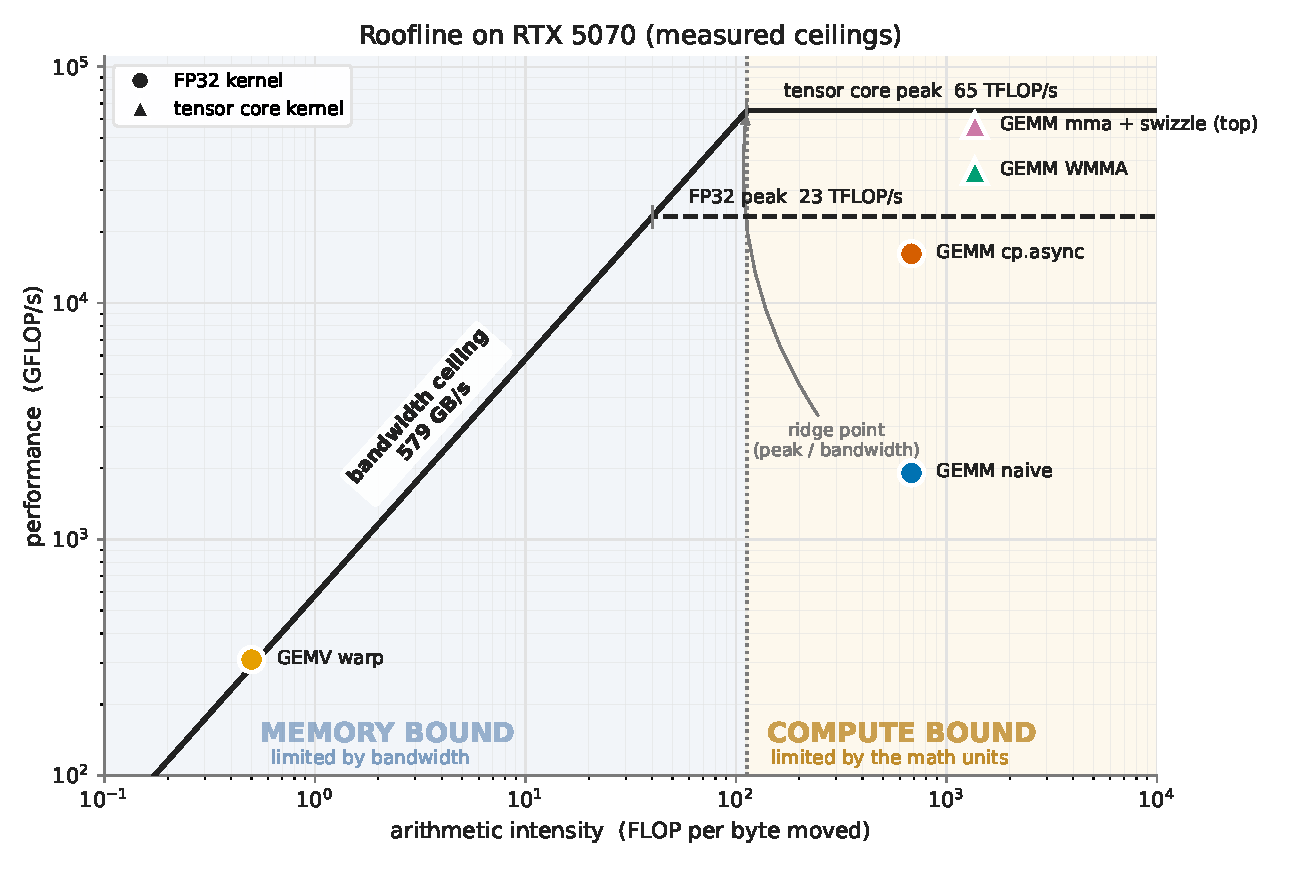
\includegraphics[width=0.95\textwidth]{roofline.pdf}
\caption{Roofline on the RTX 5070 with measured ceilings. GEMM is compute bound;
GEMV is memory bound.}
\label{fig:roofline}
\end{figure}

\section{Discussion}

The result that most shaped the work is that tiling alone loses to naive on this
card, because the large cache hierarchy makes the naive kernel's redundant traffic
cheap. Register blocking, then feeding the tensor cores through a swizzled shared
layout, are what actually move the number. The remaining ten percent to cuBLAS is
where its per shape tuning (deeper pipelines, split K for the largest shapes) lives.
The failed three stage pipeline round is kept in the engineering log as an equal
rank result: it is the honest record that a plausible change measured worse and was
reverted.

\section{Conclusion}

A hand written FP16 GEMM on the RTX 5070 reaches about 90 percent of cuBLAS and is
demonstrably compute bound, arrived at through nine logged diagnostic rounds with
one change each. The supporting families are correct and benchmarked, the roofline
is built from measured ceilings, and every number is reproducible from a clean
clone. The method, one change per round against profiler evidence, is the
transferable part.

\bibliographystyle{plain}
\bibliography{refs}

\end{document}
